% !TEX root = ../thesis.tex

\chapter{Analytická časť}
Pri strojovom učení a experimentoch je niekedy potreba na krátku dobu vyšší výkon. Pravidelne migrovanie medzi strojmi by bolo veľmi zdĺhavé. S tým nám pomôže platforma kubernetes.

Kubernetes je platforma, ktorá je veľmi robustná v nasadení, správe a orchestrácií kontajnerov. Dokáže rozdeliť súčasne záťaž medzi jednotlivými strojmi. Tato platforma v súčasnosti vytlačila predošle platformy a stala sa už štandardom. Nasadenie Kubernetes je najefektívnejšie, aj keď existuje dnes veľa podobných technológii, mnoho významných poskytovateľov ponuka klastre Kubernetes.

Podľa mojich uvážení je na našu problematiku vhodný Kubeflow.


% lorem ipsum
\section{Kubeflow}

Kubeflow ako platforma, je vhodná na nasadenie a vývoj strojového učenia. Primárne slúži pre inžinierov a vedcov, ktorý pracujú s dátami. Obsahuje viaceré komponenty, z ktorých si vývojári môžu vybrať, čo je pre ich používateľov najlepšie, čo znamená, že na nasadzovanie nie je potrebný každý jeden komponent.\cite{web}

\subsection{Architektúra}

Kubeflow stavia na Kubernetes ako systéme na nasadenie, škálovanie a správu zložitých systémov. Pomocou konfiguračných rozhraní Kubeflow, môžeme špecifikovať nástroje strojového učenia, potrebné pre náš pracovný postup. Potom môžeme nasadiť pracovný postup do rôznych cloudov, miestnych platforiem na experimentovanie a na produkčné použitie.\cite{web}
\clearpage
\begin{figure}[!ht]
    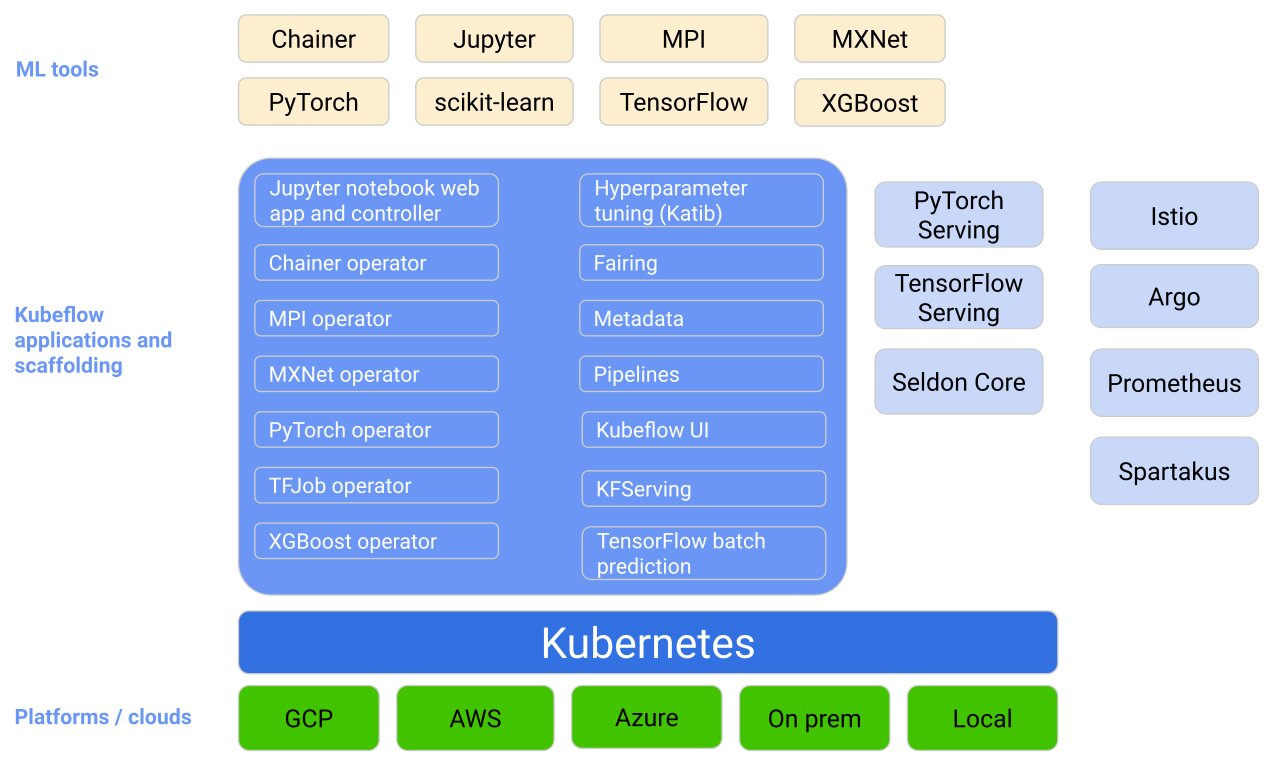
\includegraphics[width=.9\textwidth]{figures/kubeflowaarch}
    \caption{\ Architektúra kubeflow \label{o:latex_friendly_zone}}
\end{figure}
\subsection{Pracovný postup}




\section{Aliquam eu malesuada urna}

\begin{itemize}
    \item v~knihe \cite{book} autor prezentuje naozaj odvážne myšlienky
    \item nemenej zaujímavé výsledky publikuje ďalší autor v~článku \cite{article} 
    \item v~konferenčnom príspevku \cite{conference} sú uvedené tiež zaujímavé veci
    \item \LaTeX{}\footnote{\url{https://www.latex-project.org/}} je typografický jazyk
\end{itemize}

Given a set of numbers, there are elementary methods to compute its \acrlong{gcd}, which is abbreviated \acrshort{gcd}. This process is similar to that used for the \acrfull{lcm}.

\subsection{Donec vehicula consequat}
\blindtext



\subsection{Nullam in mauris consectetur}
\blindtext

\begin{lstlisting}[language=C,caption={Program, ktorý pozdraví celý svet}]
#include <stdio.h>
int main() {
    /* Print Hello, World! */
    printf("Hello, World!\n");
    return 0;
}
\end{lstlisting}


\subsection{Vestibulum tristique elementum varius}
\blindtext

\begin{table}[!ht]
	\caption{Country list}\label{t:1}
	\smallskip
	\centering

	\begin{tabular}{ |p{3cm}||p{3cm}|p{3cm}|p{3cm}|  }
		\hline
		\multicolumn{4}{|c|}{Country List} \\
		\hline
		Country Name or Area Name& ISO ALPHA 2 Code &ISO ALPHA 3 Code&ISO numeric Code\\
		\hline
		Afghanistan & AF & AFG & 004\\
		Aland Islands & AX & ALA & 248\\
		Albania & AL & ALB & 008\\
		Algeria & DZ & DZA & 012\\
		American Samoa & AS & ASM & 016\\
		Andorra & AD & AND & 020\\
		Angola & AO & AGO & 024\\
		\hline
	\end{tabular}
\end{table}


\section{Phasellus id pretium neque}
\blindtext

\blindtext
